\chapter{Inverse Probability of Treatemnt Weighting}
本章笔记均为书面形式,只汇总概要,具体内容看书面笔记.

\section{Intuition for IPTW}
\subsection{IPTW的计算方法}
\subsection{IPTW的作用}
\begin{itemize}
	\item \r{IPTW的作用:}对每一种X的取值(在Propensity score相同的subjects中),令treated subjects的counting和control subjects的counting相等.
\end{itemize}
	
	
\section{More intuition for IPTW}
这一节课的重点在于理解Pseudo-population的含义、作用,以及如何构建pseudo-population.

\r{Goal:} Using weihgting to create a pseudo-population where there is no confounding.

\section{Marginal structual model}
\subsection{Introduction to MSMs}
\r{MSM is a model for the mean of potential outcomes for whole population.}
\begin{itemize}
	\item Marginal:Model does not conditional on confounders(X). 也就是说模型不以X的某个取值为条件(E(Y$|$X=x)),而是遍历X的全部取值,是一种边缘(marginal)模型.
	\item Structural: 模型是针对potential outcomes建立的(E($Y^1$),E($Y^0$)),而不是Observed outcomes. 
	\item 模型针对的是whole population,而不是subpopulation.
\end{itemize}

\subsection{Linear MSM}
\subsection{Logistic MSM for binary outcome}
\subsection{MSM with effect modification}
\begin{itemize}
	\item Model includes effect modifiers V. V is a variable that modifies the effect of A. For example, V could be \r{diabetes, sex, race,...}, these variables could change the effect of treatment. \g{That means in different value of V, causal effect are different.}
\end{itemize}

\subsection{General MSM}
\subsection{Key issue of MSM}
建立MSM的难点在于模型是针对potential outcomes建立的,然而实际上我们只能获取observed outcome,如何在值给定observed outcome的情况下估计模型的参数?


\section{IPTW estimaion}
这一节主要讲述如何估计Marginal structual model中的参数.
\subsection{Recall: Estimation in linear regression model}
\subsection{Difference between MSM and regression model}

\begin{itemize}
	\item 若建立regression model来估计A的causal effect,模型为
	\begin{equation}
	g(E(Y|A))=\psi_0+\psi_1 A.
	\end{equation}
	此时我们估计的是$E(Y|A)=g^{-1}(\psi_0+\psi_1 A)$,这里的A是固定的某个取值a,针对的是A=a的subpopulation.
	 
	\item MSM模型为
	\begin{equation}
	g(E(Y^a))=\psi_0+\psi_1 A
	\end{equation}
	此时我们估计的是$E(Y^a)=g^{-1}(\psi_0+\psi_1 A)$,这里的A取值未定,可以是任意的取值.
\end{itemize}

\subsection{Why different?}
MSM与regression model的区别是因为\r{confounding的存在}. 但是,我们注意到在randomized trial中$E(Y|A=a)=E(Y^a)$,也就是说randomized trial中没有confounding影响,可以拟合regression model,模型的参数就是causal effect. 

这给我们提供了一种思路:既然在randomized trial中可以拟合回归模型,那我们可以尽量去构建randomized trial,然后做回归.

\subsection{利用Pesudo-population近似randomized trials}
在4.2节中,我们知道可以使用IPTW的方法构建Pesudo-population.

\begin{itemize}
	\item Pesudo-population is free from confounding.(Under ignorability and positivity assumption)
\end{itemize}

\subsection{Steps in estimating parameters from MSM}

Issue of IPTW: 使用weighting的方法人为地扩大了population siz,使模型的error更大了.

\section{Assessing balance and Distribution of weights}
Task: 检查weighting之后covariate balance是否实现.
Goal: After weighting sample is equal to randomized trial.
\subsection{Standardized difference}
\begin{itemize}
	\item 注意是对weighting后的样本做检验,而不是原样本!
	\item 列出table one.
\end{itemize} 

\section{Distribution of weights}
\begin{itemize}
	\item large weight $\longrightarrow$ large standard error.
\end{itemize}
\subsection{Bootstrapping}
\subsection{Relationship with positivity assumption}
large weight $\longrightarrow$ very small propensity score $\longrightarrow$ very small probability to get treated $\longrightarrow$ violate positivity assumption.


\section{Remedies for large weights}
\subsection{Trimming the tails}
\subsection{Weight trunction}

%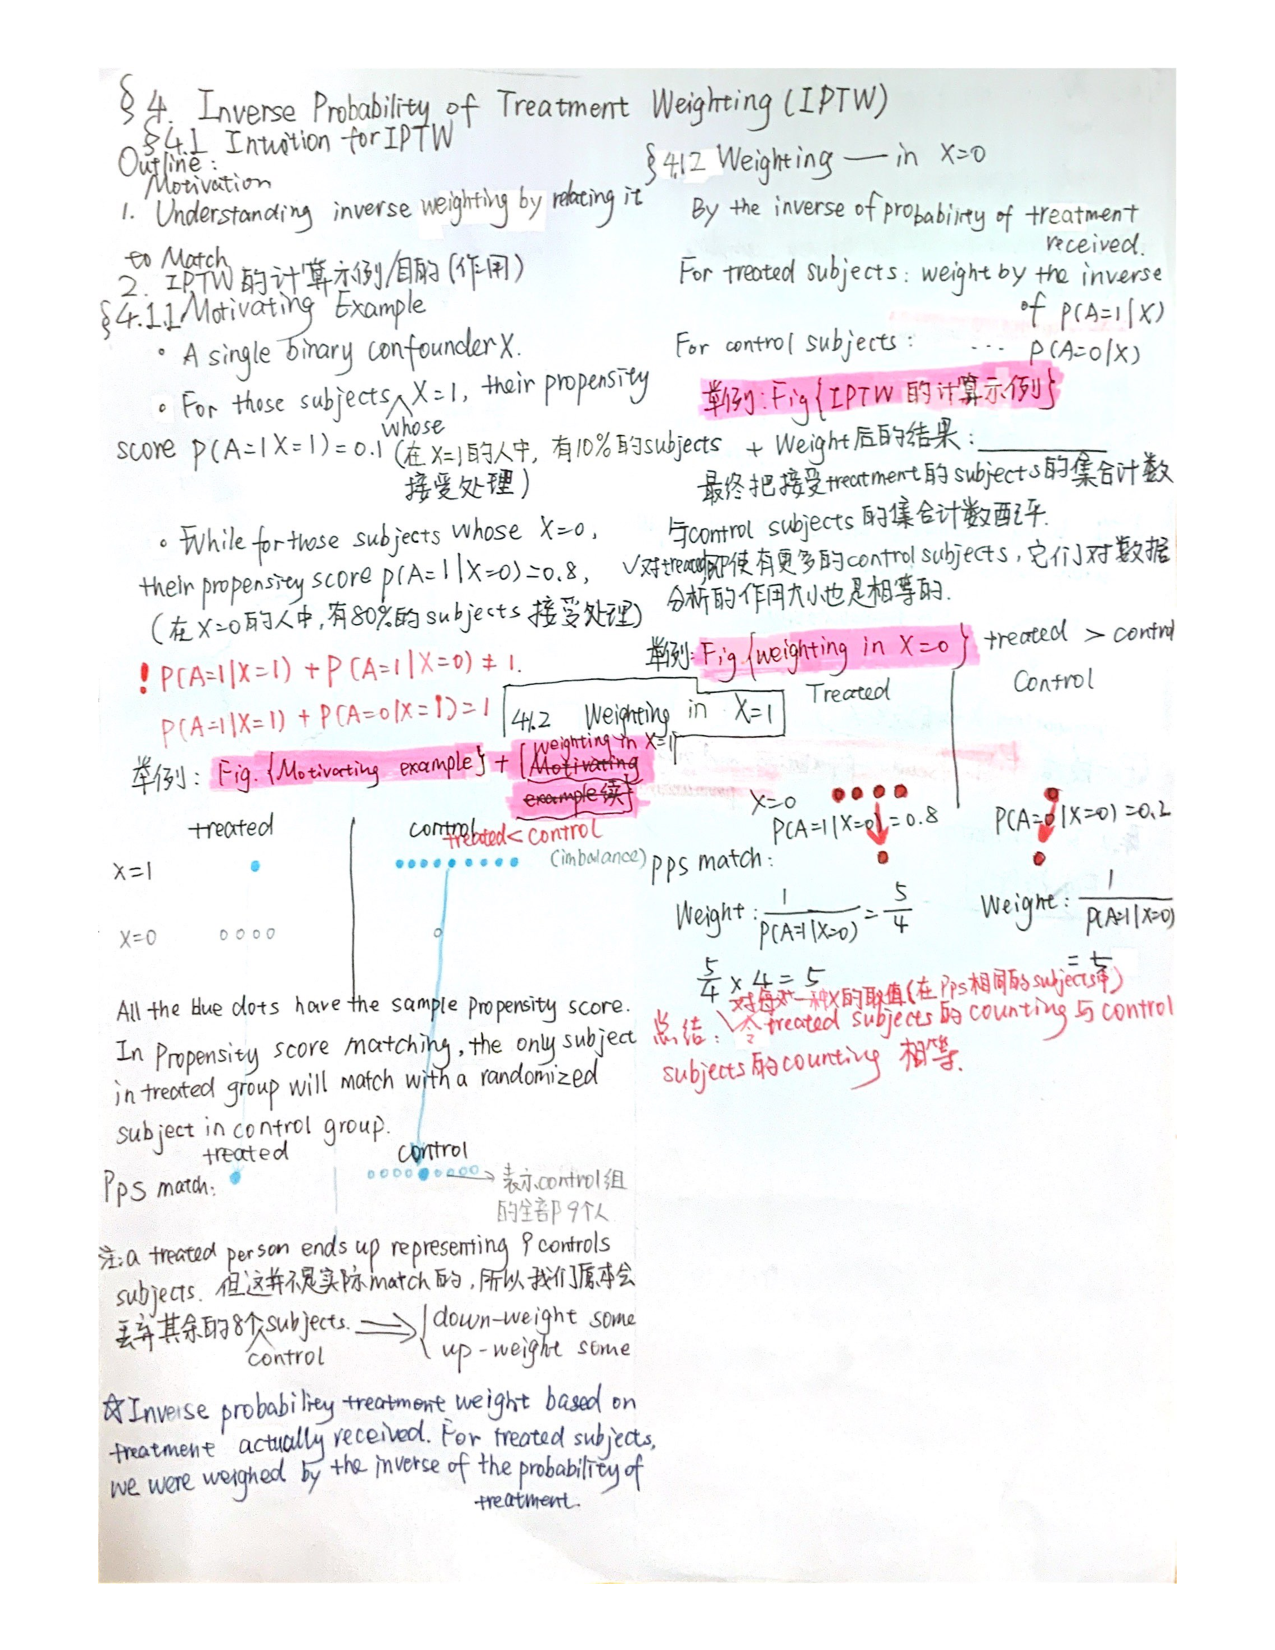
\includepdf[pages=-]{figure/4.1.pdf}
%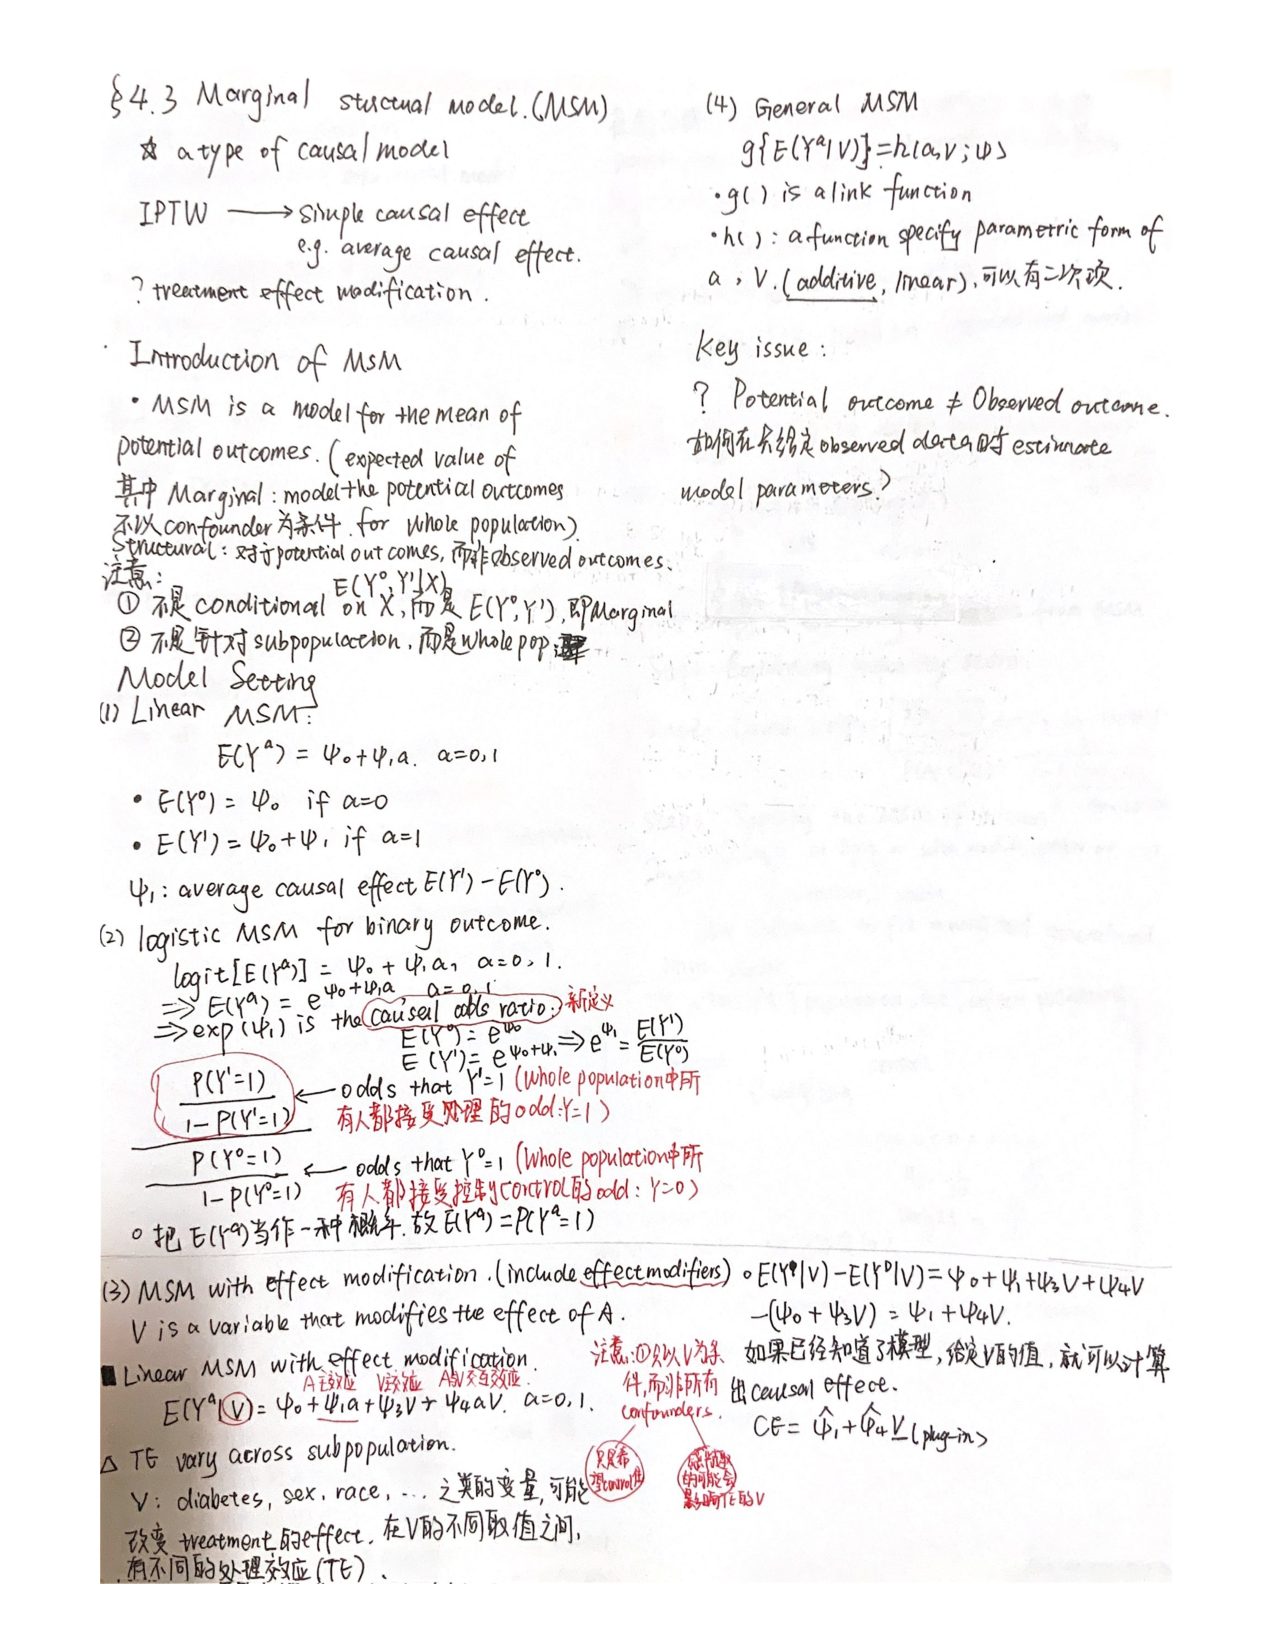
\includepdf[pages=-]{figure/4.3.pdf}
%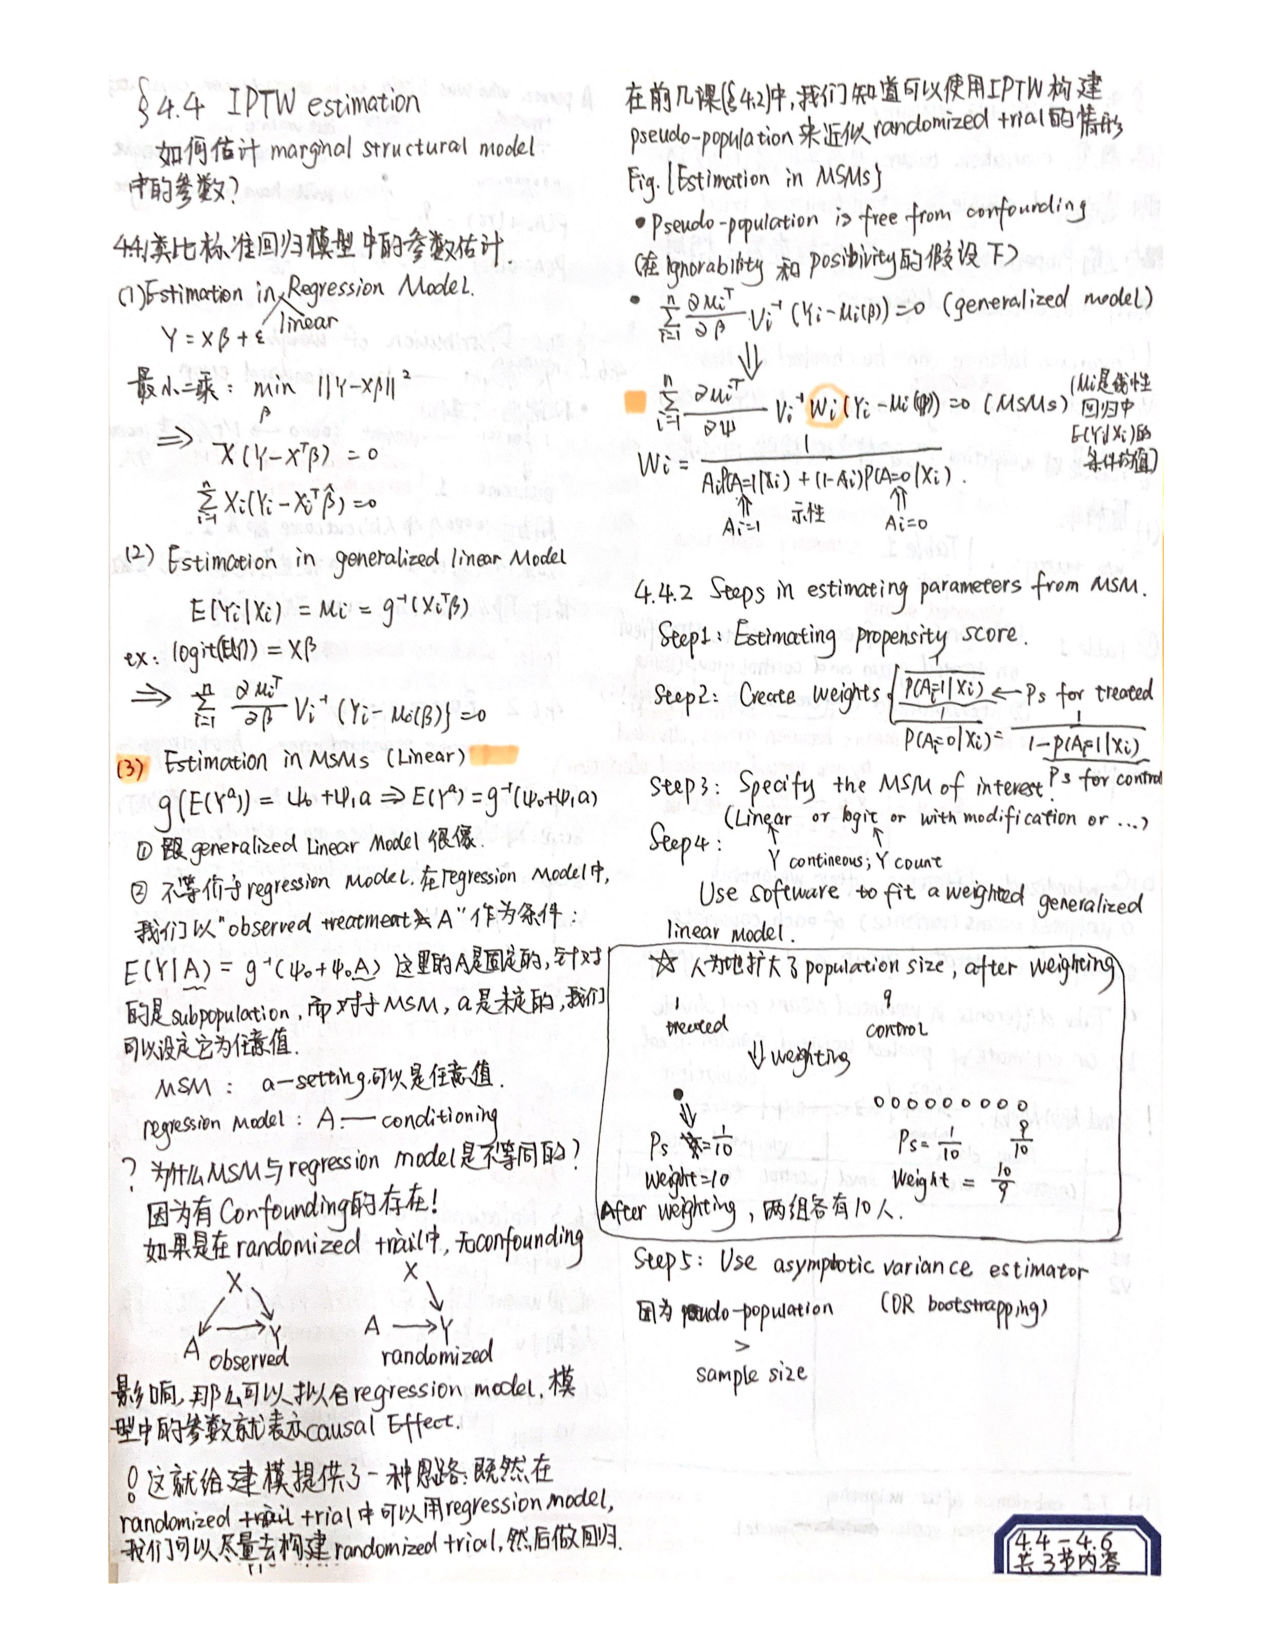
\includepdf[pages=-]{figure/4.4.pdf}
%\includepdf[pages=-]{figure/4.56.pdf}
%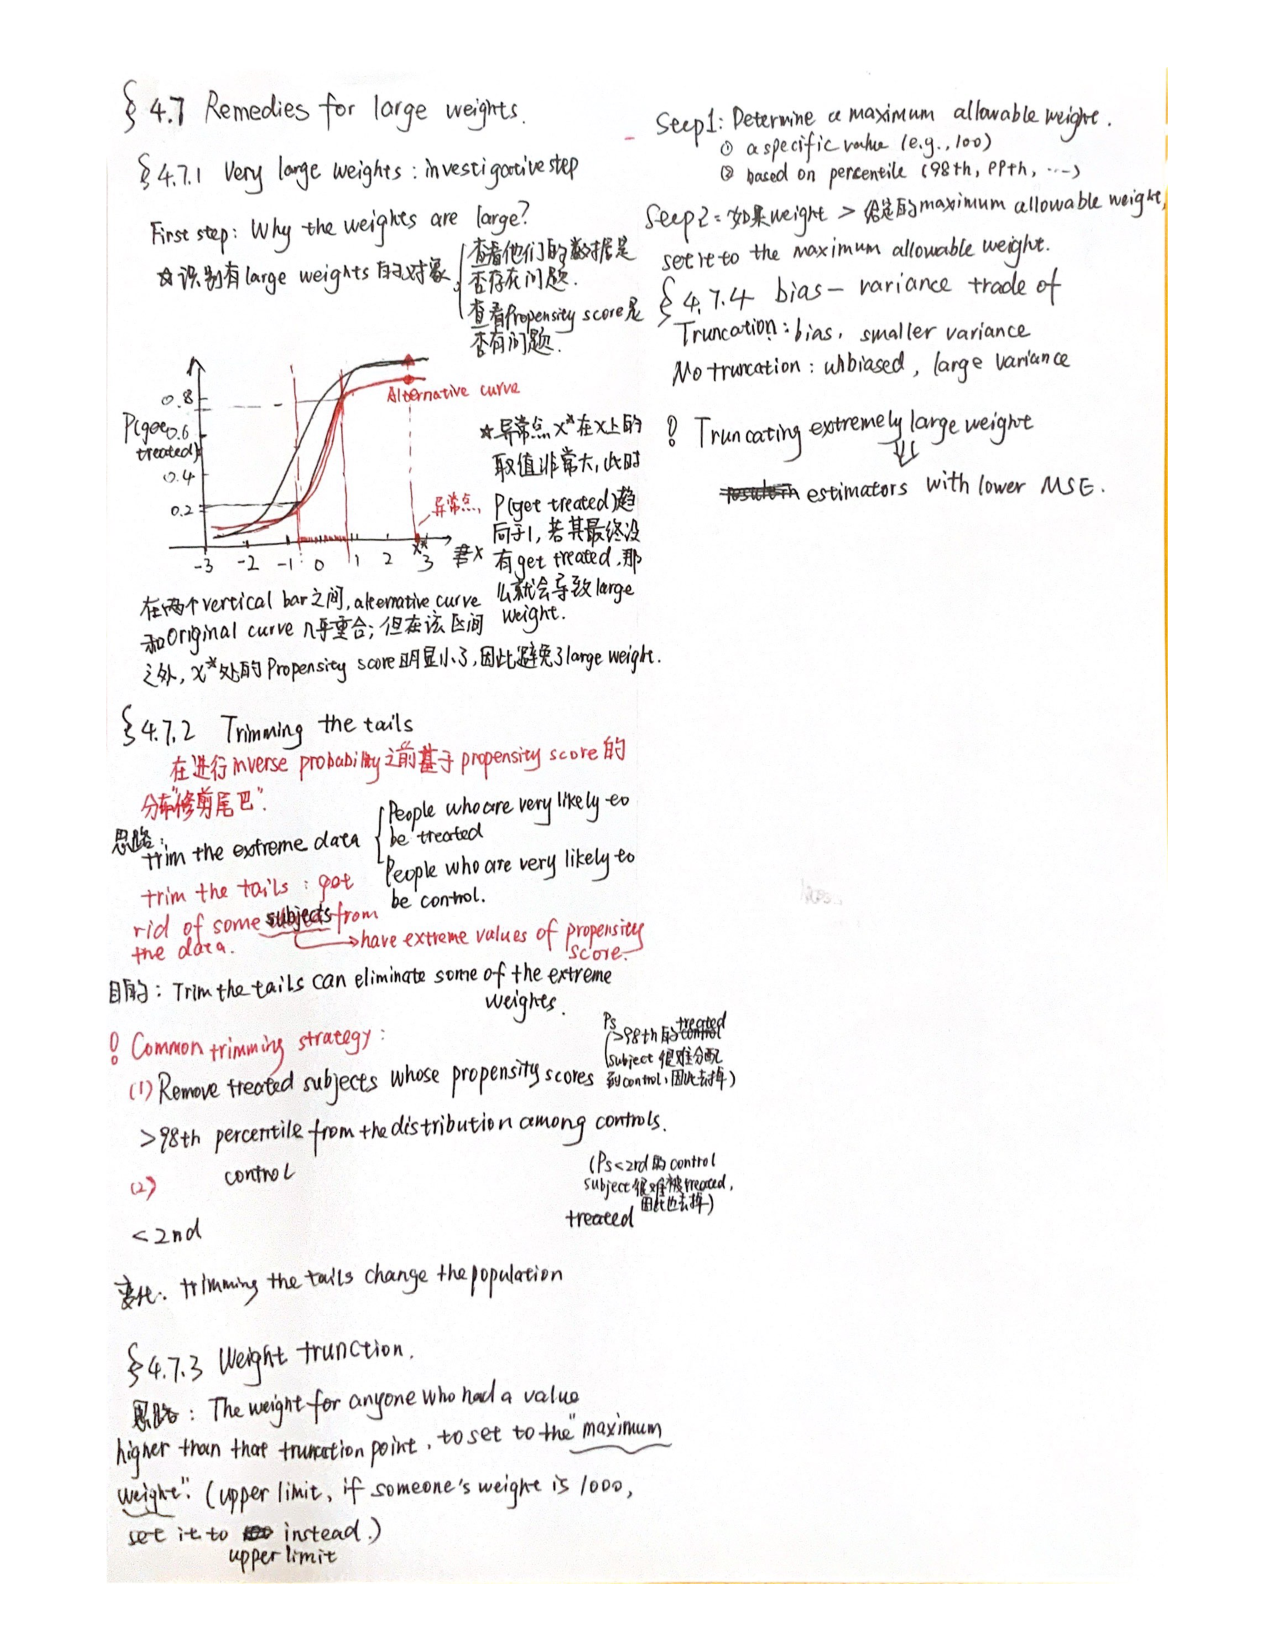
\includepdf[pages=-]{figure/4.7.pdf}